\begin{multicols} {3}
\begin{tikzpicture}
% Card
\fill[blue!20] (0,0) rectangle (3,5);
% Name
\draw (1.5,4.5) node {Msr. Roggeman};
% Mana
\draw (3,5) node[style={rectangle, fill=blue!40, very thick, minimum size=5mm}] {10};
% Health
\draw (3,0) node[style={rectangle, fill=red!40, very thick, minimum size=5mm}] {8};
% Attack
\draw (0,0) node[style={rectangle, fill=gray!40, very thick, minimum size=5mm}] {8};
% Artwork
\draw (1.5,3) node {
\includegraphics[width=2cm, height=2cm]{Images/Artwork/yves.jpg}};
% Description
\draw (1.5,1) node[align=center,text width=3cm] {\tiny{\textbf{Effect:} Whenever a student is summonded set their attack to 0.\\He wll not be taken down by them.\par}};
\end{tikzpicture}
\vfill
\columnbreak
\begin{tikzpicture}
% Card
\fill[blue!20] (0,0) rectangle (3,5);
% Name
\draw (1.5,4.5) node {Keno Merckx};
% Mana
\draw (3,5) node[style={rectangle, fill=blue!40, very thick, minimum size=5mm}] {7};
% Health
\draw (3,0) node[style={rectangle, fill=red!40, very thick, minimum size=5mm}] {6};
% Attack
\draw (0,0) node[style={rectangle, fill=gray!40, very thick, minimum size=5mm}] {5};
% Artwork
\draw (1.5,3) node {
\includegraphics[width=2cm, height=2cm]{Images/Artwork/keno.jpg}};
% Description
\draw (1.5,1) node[align=center,text width=3cm] {\tiny{\textbf{Effect:} Give ALL students +2/+2.\\He wants them to be succesfull.\par}};
\end{tikzpicture}
\vfill
\columnbreak
\begin{tikzpicture}
% Card
\fill[blue!20] (0,0) rectangle (3,5);
% Name
\draw (1.5,4.5) node {TD a la Jefke};
% Mana
\draw (3,5) node[style={rectangle, fill=blue!40, very thick, minimum size=5mm}] {4};
% Artwork
\draw (1.5,3) node {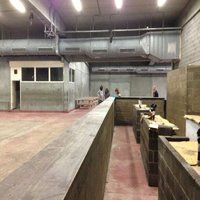
\includegraphics[width=2cm, height=2cm]{Images/Artwork/jefke.jpg}};
% Description
\draw (1.5,1) node[align=center,text width=3cm] {\tiny{\textbf{SPELL}\\ All students become inmune and have +5 attack this turn\par}};
\end{tikzpicture}
\end{multicols}